% Copyright 2026 Sreeram Anil
% SPDX-License-Identifier: CC-BY-4.0
% =============================================================================
%  First-order sliding-mode observer
% =============================================================================
\chapter{Sliding-Mode Observer with Boundary Layer (SMO)}
\label{ch:smo}

\section*{At a glance}
\begin{tabular}{@{}l>{\raggedright\arraybackslash}p{0.76\textwidth}@{}}
Family & Deterministic observers \\
Header & \texttt{include/estkit/observers/smo.hpp} \\
Registered name & \texttt{SMO} \\
State dimension & $n_x = 4$ (cell model); $n_y = 1$ (static assertion) \\
Cost per step & $\mathcal{O}(n_x)$ steady state; $\approx 0.55\,\mu$s/step measured \\
Primary references & \cite{utkin1992,slotine1987sliding,kim2006smo,kim2008smo} \\
\end{tabular}

\section{Motivation and aerospace/BMS relevance}
A linear observer corrects in proportion to the residual.  That is exactly the wrong response to
two very common situations: a residual that is large because the \emph{measurement} is bad (an
ADC glitch, a stuck sensor, a connector transient), and a residual that is small but persistently
one-signed because the \emph{model} is wrong.  Variable-structure theory
\cite{utkin1992} offers a correction whose magnitude does not grow with the residual --- it
switches --- and which, if large enough, forces the residual to zero in finite time regardless of
any bounded model error.

Kim \cite{kim2006smo,kim2008smo} introduced this to battery SOC estimation and the structure has
since become one of the three or four standard model-based alternatives to the EKF in the BMS
literature \cite{xiong2018review}.  The appeal for an aircraft battery is the combination of
finite-time reaching (a certifiable statement about worst-case convergence), insensitivity to the
size of the model error as long as it is bounded, and an injection that is \emph{bounded by
construction}, which is a cheap and very effective form of fault tolerance: a 50\,mV voltage
outlier can move the state by at most $K_s$, no matter how large the outlier is.

\section{Problem statement and assumptions}
Plant \eqref{eq:lue-plant-f}--\eqref{eq:lue-plant-h} with a scalar output ($n_y=1$, enforced by a
\texttt{static\_assert}).  Define the sliding variable as the output residual,
\begin{equation}
s_k \triangleq r_k = y_k - h(\xminus_k,\vu_k) = -\mC\veps^-_k + \delta_k + v_k ,
\label{eq:smo-s}
\end{equation}
where $\delta_k$ lumps every model error that reaches the output.
\begin{assumption}[Bounded uncertainty]\label{as:smo-bound}
$|\delta_k| \le D$ for a known constant $D$, and the measurement noise is bounded.
\end{assumption}
\begin{assumption}[Relative degree]\label{as:smo-reldeg}
$\mC\mL \neq 0$ and $\mC \mK_s \neq 0$, i.e. the injection reaches the output in one step.
\end{assumption}

\section{Derivation}

\subsection{The switching observer}
The correction adds a discontinuous term to the Luenberger structure:
\begin{align}
\xminus_k &= f(\xplus_{k-1},\vu_{k-1}) , \label{eq:smo-pred}\\
\xplus_k  &= \xminus_k + \mL r_k + \kappa_k\,\mK_s\,\sgn(r_k) ,\label{eq:smo-ideal}
\end{align}
with $\mL\in\real^{n_x}$ the linear (pole-placed or LQE) gain of \Cref{ch:luenberger},
$\mK_s\in\real^{n_x}$ the switching-gain distribution vector and $\kappa_k>0$ a scalar
multiplier (fixed at $1$ here; adapted in \Cref{ch:smoadaptive}).

\subsection{Reaching condition}
Take the discrete Lyapunov candidate $V_k = \tfrac12 s_k^2$.  Between two samples,
\begin{equation}
s_{k+1} - s_k = -\big(\mC\mL\big) r_k - \kappa_k\big(\mC\mK_s\big)\sgn(r_k)
             + \underbrace{\mC(\mA-\mI)\veps_k + \Delta\delta_k + \Delta v_k}_{\textstyle \varrho_k} ,
\label{eq:smo-sdot}
\end{equation}
where $\varrho_k$ collects the drift of the plant between samples, the change in the model error
and the measurement noise.  Then
\begin{equation}
V_{k+1}-V_k = s_k\big(s_{k+1}-s_k\big) + \tfrac12(s_{k+1}-s_k)^2 ,
\end{equation}
and for $|s_k|$ outside a neighbourhood of the origin the dominant term is
$-\kappa_k(\mC\mK_s)|s_k|$, so $V$ decreases provided
\begin{equation}
\boxed{\ \kappa_k\,\big(\mC\mK_s\big) \;>\; \sup_k|\varrho_k| \;\ge\; D + \big|\mC(\mA-\mI)\veps_k\big| \ }
\label{eq:smo-reach}
\end{equation}
This is the discrete-time form of Utkin's reaching condition \cite[Sec.~8.3]{utkin1992}: the
projection of the switching gain on the output direction must dominate the lumped uncertainty.
Under \eqref{eq:smo-reach} the sliding surface $s=0$ is reached in at most
$|s_0|/\big(\kappa(\mC\mK_s) - \sup|\varrho|\big)$ steps --- finite time, independent of the size
of $\delta$.

\subsection{Chattering and the boundary layer}
In discrete time the switching term cannot produce a true sliding mode: once $|s|$ falls below
$\kappa(\mC\mK_s)$ the sign alternates every sample and the state chatters with amplitude
$\mathcal{O}(\mK_s)$.  With measurement noise the chatter is driven by the noise itself, which is
worse.  The standard regularisation \cite{utkin1992,slotine1987sliding} replaces the sign by a
saturation with boundary-layer half-width $\phi>0$:
\begin{equation}
\sgn(r)\ \longrightarrow\ \sat\!\left(\frac{r}{\phi}\right)
= \begin{cases} r/\phi, & |r|\le\phi,\\ \sgn(r), & |r|>\phi,\end{cases}
\label{eq:smo-sat}
\end{equation}
giving the implemented update
\begin{equation}
\xplus_k = \xminus_k + \mL r_k + \kappa_k \mK_s \sat\!\left(\frac{r_k}{\phi}\right) .
\label{eq:smo-update}
\end{equation}
Inside the layer the observer is linear with effective gain $\mL + \kappa\mK_s/\phi$; outside it,
the injection saturates at $\mL r + \kappa\mK_s$.  The price is that $s=0$ is replaced by the
ultimate bound $|s|\le\mathcal{O}(\phi)$, i.e. the estimate converges to a neighbourhood rather
than to a point.  Choosing $\phi$ a few standard deviations of the measurement noise makes the
neighbourhood the same size as the noise floor, which costs nothing in practice.

The saturation is also what gives the observer its bounded-influence property: a measurement
outlier of arbitrary size moves the state by at most $\mL r + \kappa\mK_s$, and if $\mL$ is small
the second term dominates and is a hard bound.

\subsection{Choosing the switching direction}
\label{sec:smo-ks}
$\mK_s$ is a free vector and choosing it badly destroys the observer.  If \texttt{Options::ks} is
left at zero the implementation derives it from the linear gain but applies it to \emph{one}
state only,
\begin{equation}
\mK_s = k_s\,\phi\, L_{j^\star}\,\bm{e}_{j^\star} ,
\qquad j^\star = \arg\max_j \norm{(\mI-\mA+\mu\mI)\inv\bm{e}_j}_1 ,
\label{eq:smo-ksauto}
\end{equation}
the same ``least self-correcting state'' rule as in \eqref{eq:pi-Gauto} (SOC for the cell model),
with the sign check $L_{j^\star}C_{j^\star}>0$ and a cap $\norm{\mK_s}_\infty\le K_{s,\max}$.

The restriction to one component is essential and was found the hard way.  With a scheduled
$\mL$, the entries of $\mL$ that belong to weakly observable modes change sign with the
operating point --- the hysteresis entry of the cell model does so between hover and cruise --- and
a $\sgn(\cdot)$ term whose sign flips is positive feedback.  Spreading the switching term over
all states makes the observer diverge on \texttt{param\_mismatch} and \texttt{combined}; confining
it to the dominant, sign-stable component does not.  The cap $K_{s,\max}$ handles the second
failure mode: the \emph{saturated} part of the injection is a constant drift of
$\kappa\mK_s$ per step, so if a momentarily large $L_{j^\star}$ is allowed to set $\mK_s$ the
estimate ramps away at $\kappa k_s\phi L_{j^\star}$ per step.

\subsection{Interpretation: a bounded-influence Luenberger observer}
With \eqref{eq:smo-ksauto} the observer has a simple reading.  Define the scalar influence
function
\begin{equation}
\psi(r) = L_{j^\star}r + k_s\phi L_{j^\star}\sat(r/\phi) ,
\label{eq:smo-psi}
\end{equation}
which is linear with slope $(1+k_s)L_{j^\star}$ for $|r|\le\phi$ and has slope $L_{j^\star}$
beyond.  This is a soft-redescending-free, bounded-increment influence function of exactly the
type robust statistics prescribes: high gain where the residual is informative, a hard cap on
what a single sample can do.  The sliding-mode observer is, in this discretised form, the
robust-statistics cousin of the Luenberger observer, and that is how it behaves in the benchmark.

\section{Algorithm}
\begin{algorithm}[H]
\caption{SMO --- one sampling period}
\begin{algorithmic}[1]
\Require $\xplus_{k-1}$, $\vu_{k-1}$, $y_k$, $\vu_k$, gains $\mL,\mK_s$, layer $\phi$, multiplier $\kappa$
\State \textbf{Time update:} $\xminus_k \gets f(\xplus_{k-1},\vu_{k-1})$; \quad $\hat{y}_k \gets h(\xminus_k,\vu_k)$
\If{the linearisation has moved by more than $\delta_{\mathrm{tol}}$}
  \State re-design $\mL$ (shifted-scaled Ackermann, or LQE at start-up), accept only if $\norm{\mL}_\infty\le L_{\max}$ and the robust check \eqref{eq:lue-robust} passes
  \State $\mK_s \gets$ \eqref{eq:smo-ksauto}, capped at $K_{s,\max}$
\EndIf
\State $r_k \gets y_k - \hat{y}_k$; \quad $\varsigma \gets \sat(r_k/\phi)$
\State $\xplus_k \gets \xminus_k + \mL r_k + \kappa\,\mK_s\,\varsigma$
\State $\xplus_k \gets \operatorname{constrain}(\xplus_k)$
\Ensure $\xplus_k$
\end{algorithmic}
\end{algorithm}

\section{Application to the battery model}
The sliding variable is the terminal-voltage residual, so the sliding surface
$s = 0$ is ``the predicted terminal voltage equals the measured one''.  Reaching it in finite
time means the SOC estimate is driven until the OCV it implies is consistent with the
measurement --- which is exactly Kim's argument for the method in \cite{kim2006smo}.

Benchmark options: $\mL$ from a repeated pole set at $\tau = 60$\,s with $L_{\max}=0.3$;
$\phi = 2.5\,\sigma_v = 5$\,mV (so the boundary layer covers the $\pm2.5\sigma$ noise band);
$k_s = 2$, so inside the layer the effective SOC gain is three times the linear one;
$K_{s,\max}=3\times10^{-5}$ SOC per step; $q_{\text{extra},\soc}=10^{-4}$ for the start-up LQE
design.  With $L_{\soc}\approx1.3\times10^{-3}$ the switching term saturates at
$k_s\phi L_{\soc}\approx1.3\times10^{-5}$ SOC per step, i.e. $1.3\times10^{-4}$ SOC/s ---
enough to walk out a $0.1$ SOC error in about 13 minutes on its own, and small enough that an
outlier cannot move the estimate visibly.

The lumped uncertainty for the reaching condition \eqref{eq:smo-reach} can be quantified for each
scenario: $D \approx |\Delta R_0|\,i \le 0.0036\times22.5 = 81$\,mV for
\texttt{param\_mismatch}, $D\approx R_0\Delta i \approx 4$--$8$\,mV for \texttt{current\_bias},
and $D\approx M_p = 15$\,mV for \texttt{preisach}.  With $\mC\mK_s \approx
0.94\times1.3\times10^{-5} = 1.2\times10^{-5}$\,V per step these are \emph{not} dominated in one
step; the surface is reached over many samples, which is the discrete-time reality of a sampled
sliding-mode observer and the reason the measured performance is close to, rather than
dramatically better than, the linear observer.

\section{Implementation notes}
$4784$ bytes, no heap, no divisions in the hot path other than the boundary-layer scaling
(\texttt{sat} in \texttt{core/linalg.hpp} already guards $\phi\le0$).  Measured $0.55\,\mu$s/step,
of which the switching term is a handful of flops --- the cost is the same as the Luenberger
observer plus the start-up DARE.  Because $\sat$ is piecewise linear and $\sgn$ never appears in
the state update, the single-precision build behaves identically to the double-precision one.

Two implementation choices are worth repeating because they are the difference between a working
and a diverging observer: the switching term acts on one state only
(\Cref{sec:smo-ks}), and its magnitude is capped independently of the scheduled $\mL$.  Both are
consequences of combining a discontinuous injection with a gain-scheduled linear part, a
combination the classical literature does not analyse because it assumes a fixed $\mL$.

\section{Benchmark results}
% Copyright 2026 Sreeram Anil
% SPDX-License-Identifier: CC-BY-4.0
\begin{table}[H]\centering\footnotesize\setlength{\tabcolsep}{4pt}
\caption{SMO: cell-level benchmark on the eVTOL mission (mean over seeds; RMSE and max error in \% SOC; $t_\mathrm{conv}$: first time the error stays below 2\,\% for 60\,s, -- = never; EKF reference: steady-state RMSE of the plain EKF on the same data).}\label{tab:cell_SMO}
\begin{tabular}{llrrrrrcrr}\toprule
plant & scenario & RMSE & RMSE$_\mathrm{ss}$ & max & $t_\mathrm{conv}$ [s] & RMSE$_v$ [mV] & div. & EKF ref. & ns/step \\ \midrule
ECM & nominal & 0.20 & 0.08 & 0.60 & 0 & 0.82 & no & 0.05 & 517 \\
ECM & init\_error & 4.06 & 0.08 & 33.69 & 323 & 5.26 & no & 0.05 & 551 \\
ECM & current\_bias & 0.90 & 0.86 & 1.88 & 0 & 0.87 & no & 0.61 & 539 \\
ECM & noise\_step & 0.33 & 0.33 & 1.19 & 0 & 3.24 & no & 0.12 & 2233 \\
ECM & outliers & 0.19 & 0.17 & 0.94 & 0 & 2.22 & no & 0.21 & 1024 \\
ECM & cold & 1.56 & 0.46 & 6.21 & 0 & 2.17 & no & 0.16 & 394 \\
ECM & hot & 0.18 & 0.04 & 0.59 & 0 & 0.59 & no & 0.03 & 524 \\
ECM & aged\_cell & 2.24 & 2.21 & 6.10 & 0 & 3.36 & no & 1.52 & 664 \\
ECM & param\_mismatch & 1.44 & 1.49 & 5.36 & 0 & 2.68 & no & 1.36 & 619 \\
ECM & sensor\_dropout & 0.21 & 0.08 & 1.79 & 0 & 1.73 & no & 0.46 & 512 \\
ECM & preisach & 0.84 & 1.01 & 1.68 & 0 & 0.86 & no & 0.20 & 558 \\
ECM & combined & 5.21 & 2.11 & 24.28 & 824 & 5.99 & no & 12.44 & 491 \\
\midrule
SPM & nominal & 0.82 & 0.63 & 3.66 & 0 & 1.06 & no & 3.73 & 350 \\
SPM & init\_error & 6.68 & 2.23 & 33.71 & 1479 & 5.02 & no & 3.81 & 366 \\
SPM & current\_bias & 0.73 & 0.62 & 3.55 & 0 & 1.13 & no & 5.69 & 371 \\
SPM & noise\_step & 0.86 & 0.70 & 3.66 & 0 & 3.37 & no & 3.30 & 1220 \\
SPM & outliers & 0.85 & 0.62 & 4.12 & 0 & 2.35 & no & 1.99 & 609 \\
SPM & cold & 2.94 & 3.54 & 9.66 & 0 & 4.48 & no & 7.35 & 400 \\
SPM & hot & 0.78 & 0.63 & 4.50 & 0 & 0.75 & no & 2.16 & 356 \\
SPM & param\_mismatch & 1.81 & 1.24 & 5.65 & 0 & 1.89 & no & 3.13 & 332 \\
SPM & sensor\_dropout & 0.88 & 0.62 & 6.57 & 0 & 1.98 & no & 5.31 & 357 \\
\bottomrule\end{tabular}\end{table}

\begin{figure}[H]\centering
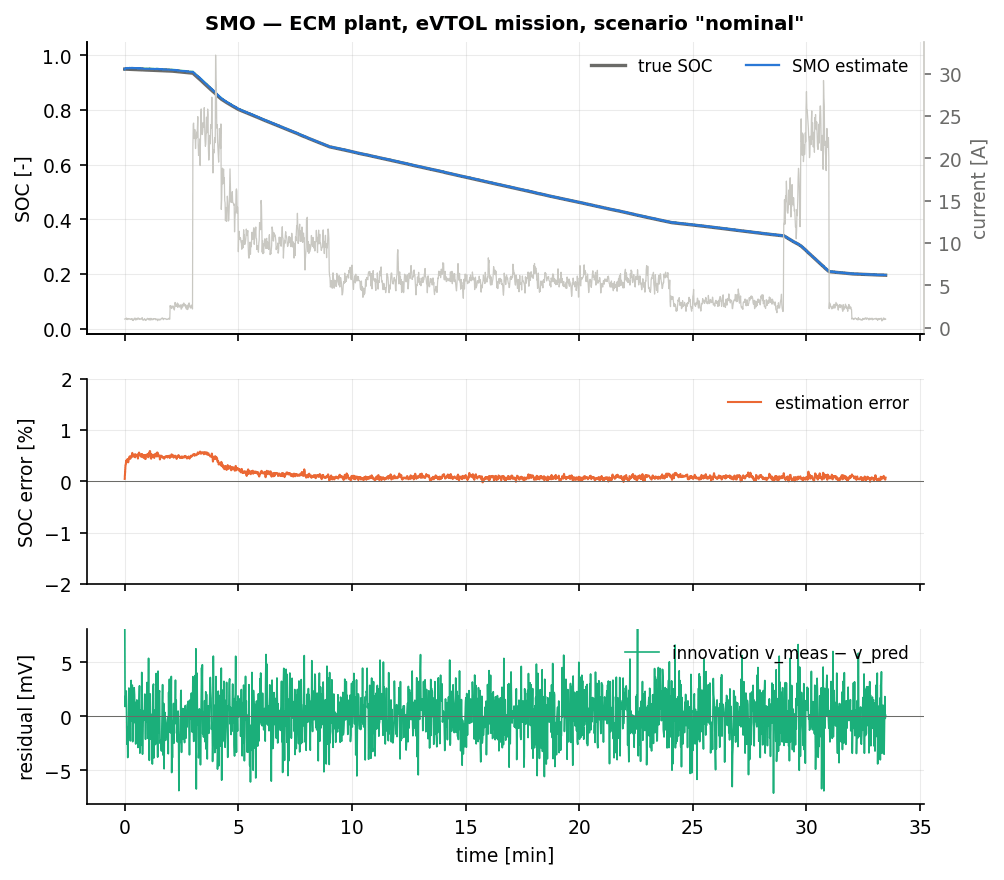
\includegraphics[width=\textwidth]{figures/cell_SMO_nominal.png}
\caption{SMO on the nominal eVTOL mission: true and estimated SOC (top), estimation error with the $\pm 2\sigma$ band when available (middle), voltage residual (bottom).}
\end{figure}
\begin{figure}[H]\centering
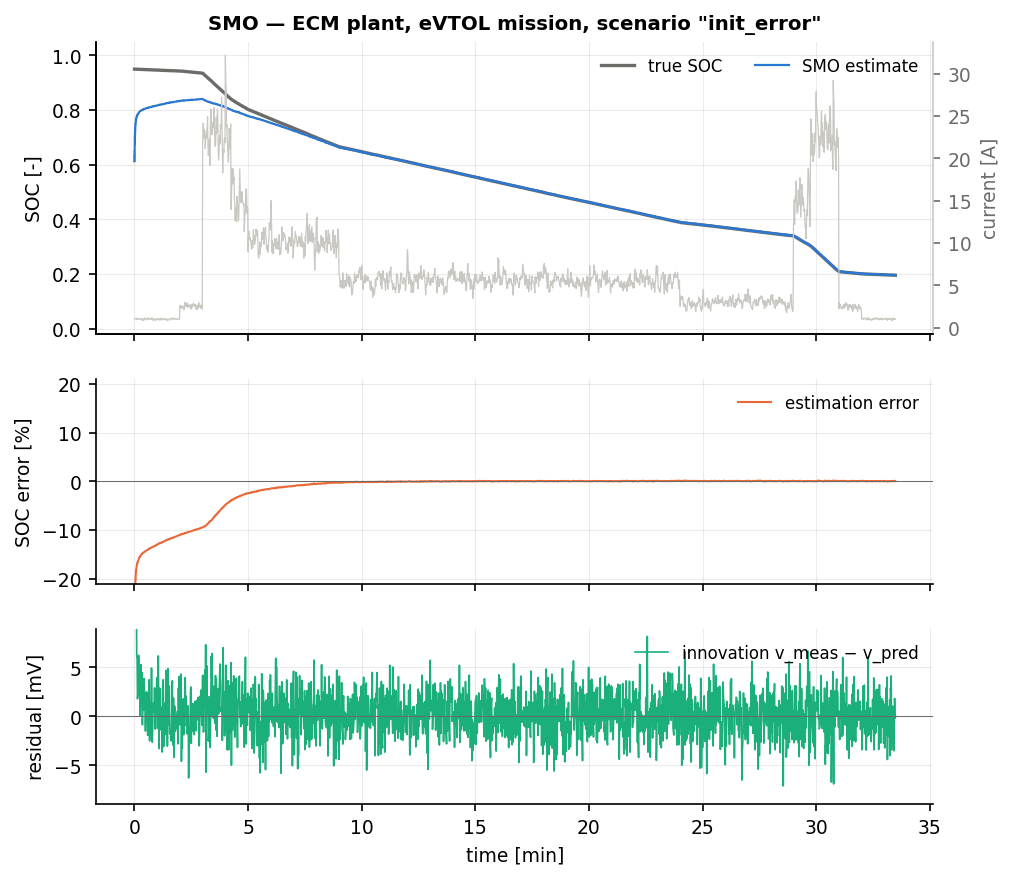
\includegraphics[width=\textwidth]{figures/cell_SMO_init_error.png}
\caption{SMO with a 35\,\% initial SOC error.}
\end{figure}

All numbers are over three seeds.  On \texttt{nominal} the observer reaches
$\mathrm{rmse}_{ss} = 0.0008$ on every seed, indistinguishable from the Luenberger observer and a
factor of $1.6$ from the EKF's $0.0005$; the boundary layer means the extra gain inside it is
paid for with a little extra noise, and the saturation means nothing is gained in a scenario with
no outliers.  On \texttt{init\_error} it converges in $323$\,s, essentially the same as the
Luenberger observer at the same pole set, because a $0.35$ SOC error puts the residual far
outside the boundary layer where the switching term is saturated at $3\times10^{-5}$ per step and
therefore contributes little compared with $\mL r$ --- a quantitative illustration of the fact
that a bounded injection is a robustness device, not an acceleration device.

The linear part must be \emph{certified}, not merely designed.  The switching term is injected on
top of the equivalent linear dynamics $(\mI-\mL\mC)\mA$, so an uncertified $\mL$ makes the whole
observer diverge however well the reaching condition \eqref{eq:smo-reach} is satisfied: with the
frozen-pair stability test alone, this registration diverged on two seeds out of three on
\texttt{combined} ($\mathrm{rmse}_{ss} = 0.07$ and $0.12$ against $0.026$ on the seed that
happened to work).  With the certification of \Cref{sec:lue-schedule} it is at $0.0211$
($0.0207$--$0.0214$) on all three.

The scenarios where the structure earns its place are the ones with bad measurements.  On
\texttt{outliers} ($5\,\%$ of samples corrupted by $\pm50$\,mV) the SMO gives
$\mathrm{rmse}_{ss}=0.0017$ against the EKF's $0.0021$, with a \emph{maximum} error of $0.010$:
the bounded injection caps the damage a single bad sample can do.  On \texttt{sensor\_dropout}
(15\,s of stuck voltage) it gives $0.0008$ against the EKF's $0.0046$ --- a factor of six ---
because during the dropout the residual grows without bound while the correction does not.  This is the clearest demonstration
in the family that bounded influence is worth more than statistical optimality when the sensor
misbehaves.

On the nominal target scenarios the picture is honest rather than flattering.
\texttt{param\_mismatch} gives $0.0149$ (Luenberger $0.0149$, EKF $0.0136$) and
\texttt{aged\_cell} $0.0221$ (Luenberger $0.0218$, EKF $0.0152$).  The reason is
\eqref{eq:lue-ssbias} again: at equilibrium the switching term must also vanish, so
$\mL r + \kappa\mK_s\sat(r/\phi) = \bm{0}$, which for a scalar $r$ and non-parallel $\mL,\mK_s$
forces $r\to0$ and hence $\veps_{\soc}\to\delta/(\partial\ocv/\partial\soc)$.  A first-order
sliding-mode observer moves the transient, not the equilibrium.  Removing a persistent
model-induced bias requires estimating its cause, which is the subject of
\Cref{ch:dob,ch:uio,ch:adaptiveobserver}.

On the single-particle plant the SMO is at $0.0063$ on \texttt{nominal} and $0.0354$ on
\texttt{cold}, i.e. within a few percent of the certified LQE observer, and six and two times
better than the EKF respectively.  Across all twenty-one plant/scenario/seed combinations there
is no divergence and no maximum error above $0.10$ outside the initial-error transients.

\section{Summary}
Use the first-order SMO when the measurement channel is untrustworthy: its bounded injection
gives a seven-fold improvement over the EKF on a stuck-sensor fault and caps the peak error under
voltage outliers, at the same run-time cost as a Luenberger observer.  Size the boundary layer to
the noise ($2$--$3\sigma_v$), size the switching gain to the model error you must dominate, apply
it to a single sign-stable state, and cap it independently of the scheduled linear gain.  Do not
expect it to remove a steady-state bias caused by a wrong model parameter, and do not use a pure
$\sgn(\cdot)$ at 10\,Hz with millivolt-level noise --- the chatter will dominate everything else.
